The CMS detector~\cite{Chatrchyan:1129810}, with a very large angular coverage around the interaction points except for the two ends of the beam line, is designed to be a general purpose particle detector.
The CMS detector is composed of solenoid magnet and steel yokes weighting 14,000 tonne, using almost twice much iron as the Eiffel Tower.
The main goal is to detect and measure precise momentum and energy of all stable particles emitting from the proton-proton collisions.

The CMS detector design and layout is driven by an important aspect, the superconducting solenoid providing an average 3.8 T magnetic filed for bending the trajectory of charged particles leaving the interaction point.
The strong but uniform magnetic fileds generated by the solenoid is parallele to the beam direction, while not interfering with the LHC beam operation.
The inner tracking system with a pixel detector and a strip tracker is positioned in the immediate proximinity of the interaction point.
The trajectory (also known as the track) of the charged particles originating from the collision points in the magnetic field can be reconstructed using the small deposits of energy left by the charged particles, while passing through the tracking system.
The energy is small enough that the momentum of the particle could be considered unchanged.
Calorimeters measuring the energy of the specific particles for particle identification are placed outside of the tracking system.
Therefore, the energy of the long-lived particle except for the muons and weakly interacting particles such as neutrinos can be deposited completely into the detector before reaching the solenoid.
Finally, the outermost muon detectors can further give measurements of precise momentum and time resolution of muons which are expected to penetrate all detector components. 

Most detector systems are confined in the region where the magnetic field generated from the solenoid is expected to be uniform, and the trajectory of muons penetrating all detector component is one key characteristic of the CMS detector and thus the name of the detector being the compact muon solenoid.
The layout of the detector can be found in Fig.~\ref{fig:cms_layout}
\begin{figure}\centering
    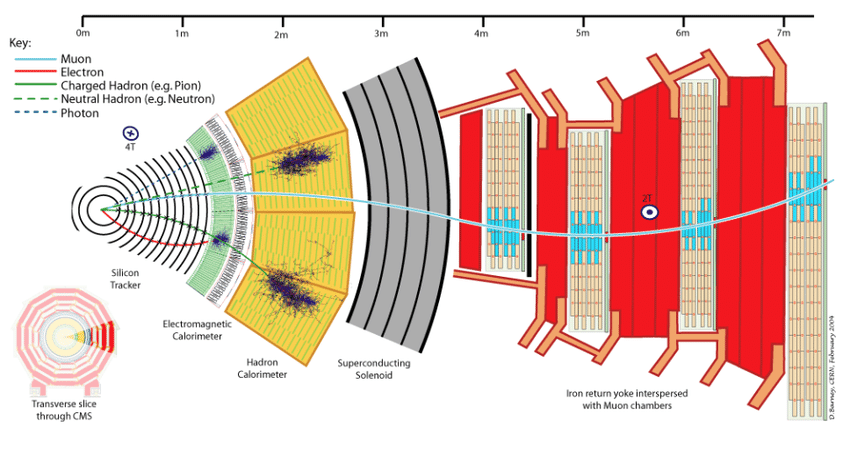
\includegraphics[width=\textwidth]{figure/cms_layout.png}
    \caption{Cross section diagram of the CMS detector and its various subdetector components.}
    \label{fig:cms_layout}
\end{figure}

\subsection{Coordinate system}
The CMS coordinate system is right-handed with its origin at the interaction points, where the $x$-axis points toward the center of the LHC ring, the $y$-axis points to the sky, and the $z$-axis points toward counterclockwise beam direction.
The coordinate consists of the transverse plane, \ie, the $xy$-plane, and the longitudinal $z$-axis.
Due to the cylindrical geometry of the CMS detector, it make sense to use a cylindrical coordinate system, where $\phi$ is an azimuthal angle in the transverse plane and $\theta$ is a polar angle between the $z$-axis, as shown in Fig~\ref{fig:cms_coord}.
\begin{figure}\centering
    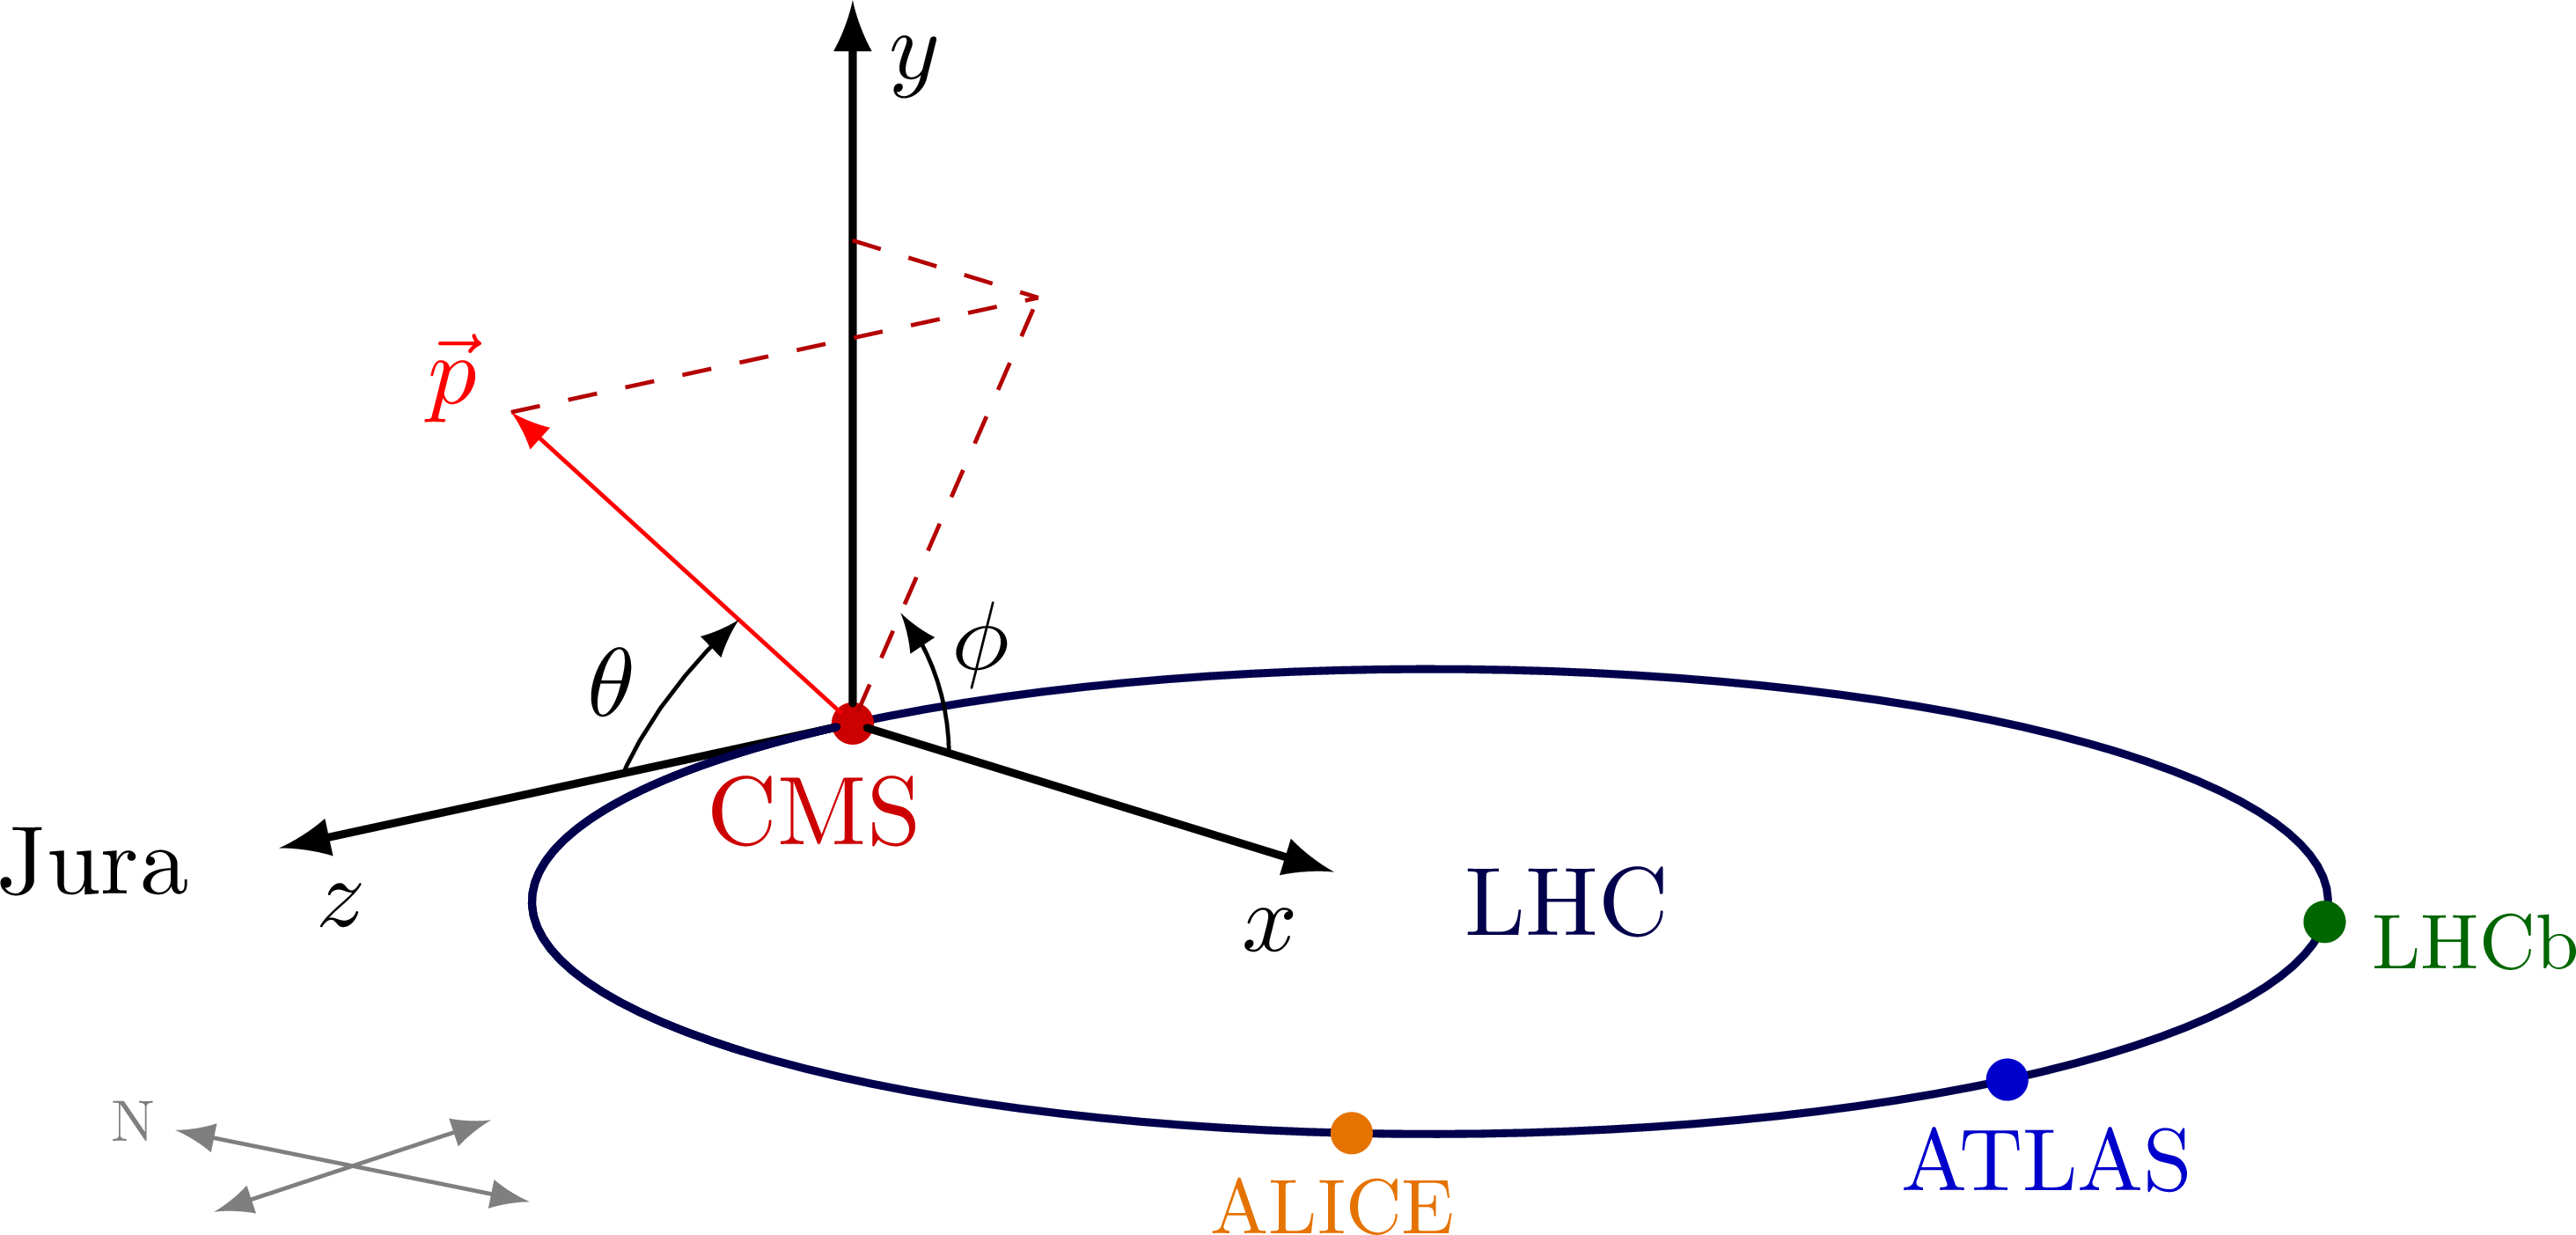
\includegraphics[width=\textwidth]{figure/cms_coord.png}
    \caption{Diagram of the coordinate of the CMS detector.}
    \label{fig:cms_coord}
\end{figure}

Due to the parton density function, the colliding partons carry unknown momenta in the beam direction, even though two protons collide from opposite directions with the same momenta at the $z$ component.
The center of mass of a hard process occurring inside the detector is likely to be boosted along the beam direction.
The polar angle separation $\delta\theta$ between two particles originating from such hard process will not be Lorentz invariant after boosted along the beam direction.
It can be expressed by an Lorentz invariant observable called rapidity as
\begin{linenomath}\begin{equation}\label{eq:cms_rap}
    y = \frac{1}{2}ln \Bigl(\frac{E+p_z}{E-p_z}\Bigr)
\end{equation}\end{linenomath}
Moreover, since the designed interaction energy in the CMS detector is very high compared with the final state particles masses, the rapidity can be further defined as pseudorapidity ($\eta$) with the low mass approximation of $E \rightarrow \vec{p}$.
The pseudorapidity is a function of the polar angle (Fig.~\ref{fig:cms_eta_theta}) defined as
\begin{linenomath}\begin{equation}\label{eq:cms_eta}
    \eta = -ln \biggl(tan\Bigl(\frac{\theta}{2}\Bigr) \biggr)
\end{equation}\end{linenomath}
where $\theta$ is the polar angle.
It is also worth mentioning that the transverse momentum $\PT=\sqrt{p^2_x+p^2_y}$ and $\phi$ are Lorentz invariant under the longitudinal boost.
That is the reason why the four-momentum is described as $(\PT, \eta, \phi, E)$ instead.
\begin{figure}\centering
    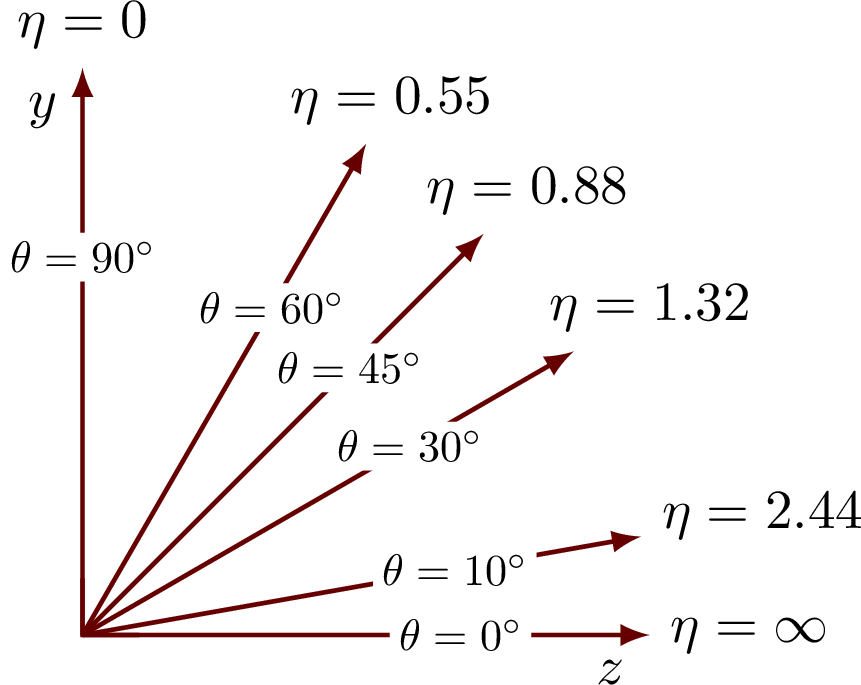
\includegraphics[width=0.7\textwidth]{figure/cms_eta_theta.png}
    \caption{Diagram showing the conversion between $\theta$ (in degrees) and $\eta$.}
    \label{fig:cms_eta_theta}
\end{figure}

\subsection{Tracking system}
The measurement of the momentum of particles plays an important role in helping us to build up a picture of what happens in the collisions.
The transverse momentum, \PT, of a particle can be calculated by tracking its path through a magnetic field as
\begin{linenomath}\begin{equation}\label{eq:cms_momentum}
    \PT = qrB
\end{equation}\end{linenomath}
where $q$ is the electric charge of the charged particle and $r$ is the radius of its trajectory under the magnetic field $B$.
The more curved the path, the less momentum the particle had.
The tracking system is designed to reconstruct the trajectory of charged particles by recording the positions of the small energy deposits left by charged particles passing through the detector components, including high-energy muons, electrons, hadrons, and tracks coming from the decay of short-lived particles such as \PQb quarks.
In order to record particle paths accurately yet with minimum energy loss so as to disturb the particle as little as possible, the trackers use just a few measurement points to reconstruct the tracks.

The measurement is silicon based to resist radiation and is accurate to 10 micrometer, a fraction of the width of a human hair.
The silicon sensors are composed of high does p-type backplane with high reverse bias voltage placed below the bulk which induce electron-hole pairs while high energy charged particles passing through the depletion region.
The electron-hole pairs are carried out to surface through the reverse bias voltage and create a small current which is the signal via additional electronic circuits.
The detector modules composed of silicon-based equipment manufactured on 2D wafers are positioned around the interaction point to have a good coverage of all the particles originating from the collisions.
The final design a tracker consists of the pixels, at the very core of the detector and dealing with the highest intensity of particles, and the silicon microstrip detectors that surround it.
The sensor components in the pixel detectors are manufactured in $100 \times 150 \mu$m cells.
In contrast, the strip trackers are composed of sensor manufactured in 120 - 180 $\mu$m wide strips stretching across an entire module, thus having lower granularity than the pixel detectors.
Though it would be ideal to have full 2D information for each module, it would be practical to lower the power density, which requires more cooling system introducing much more material that would alter the particle trajectory.

\begin{figure}[H]\centering
    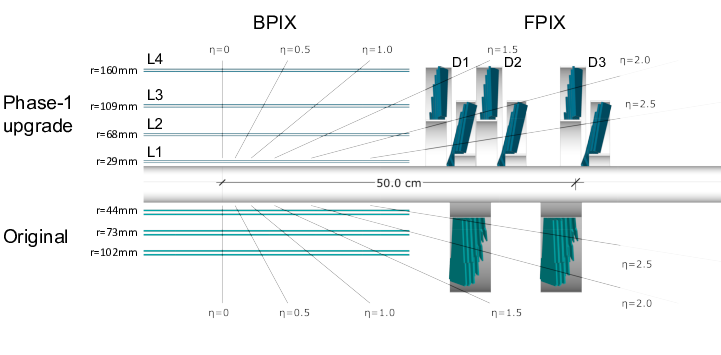
\includegraphics[width=0.9\textwidth]{figure/cms_pixel.png}
    \caption{Arrangement of the Pixel detector after phase 1 upgrade and the original one.}
    \label{fig:cms_pixel}
\end{figure}

The pixel detectors are situated closest to the interaction point and can be separated into two parts, one is composed of three barrel layers (BPix) and the other one is with two endcap disks (FPix).
The layout of the pixel detectors has been modified since the phase-1 upgrade in 2017~\cite{CMSTrackerGroup:2020edz} into four layers in the barrel part and six disks in the endcap part, as shown in Fig.~\ref{fig:cms_pixel}.
The original design can provides 3 tracking points, after the upgrade, the arrangement can further offer 4 tracking points even in high pileup environment.
The BPix having a radial distance of 2.9, 6.8, 10.9, 16.0 cm from the interation points provide high resolution starting points for the algorithm to reconstruct the particle trajectories.
The FPix situated at $|z|$ positions 30.9, 33.8 38.4, 41.3 47.9, 50.8 cm, covering 6.5 cm of radial distance from the beam axis, giving the pixel modules and angular coverage up to $|\eta|<2.5$ around the interaction point.

\begin{figure}[H]\centering
    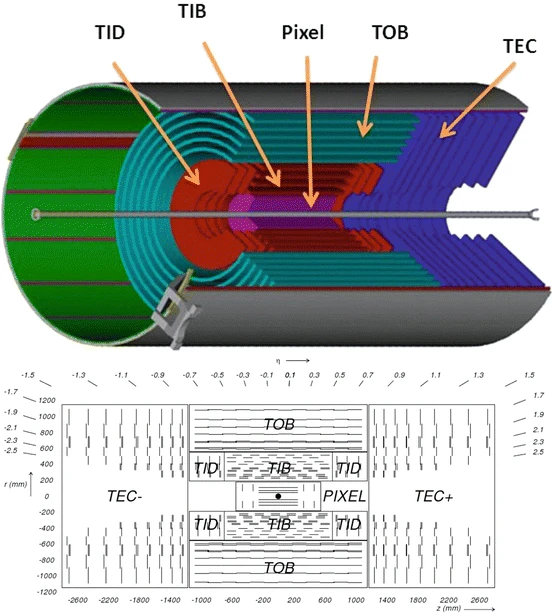
\includegraphics[width=0.8\textwidth]{figure/cms_tracker.png}
    \caption[Schematic overview and $r-z$ view (bottom) of the CMS tracking system.]{
        Schematic overview (top) and $r-z$ view (bottom) of the CMS tracking system.
        The silicon pixel detector in the center is surrounded by the strip detector which consists of endcaps and different barrel components.
    }
    \label{fig:cms_tracker}
\end{figure}
The strip detectors are situated outside the pixel system with 5.5 m in length, 2.4 m in diameter and angular coverage up to $|\eta|<2.5$, as shown in Fig.~\ref{fig:cms_tracker}.
It contains two barrel part occupying a radial coverage from 25.5 to 108.0 cm over the 10 layers of strip modules between the tracker inner barrel (TIB) and the tracker outer barrel (TOB) system, and two endcap part extending the coverage in the $|z|$ directions to 282 cm and angular coverage up to $|\eta|<2.5$ with 13 layers of strip modules between the tracker inner disks (TID) and tracker endcaps (TEC).
There are 9.6 million $p^+$ strips implanted into n-type bulks with 320 $\mu$m thickness inside the strip tracker.
The positive voltage is connected with the n-type backplane of the bulk to produce a reverse bias voltage between the backplane and $p^+$ strip.

\subsection{Electromagnetic calorimeter (ECAL)}
The ECAL detector mounted outside the tracker system is designed to measure the electromagnetic deposit energy of photons and electrons under strong magnetic field.
It is composed of 75 848 homogeneous lead tungstate (PbWO$_4$) crystals with photodetectors, as shown in Fig.~\ref{fig:cms_crystal}.
The photodetectors can capture the signal when the charged particles pass through and excite the crystal atoms, subsequently releasing the excitation energy in narrow frequency photon shower.
Due to the short radiation length (0.89 cm), small Molière radius (2.2 cm), the lead tungstate is chosen as the scintillating crystal to provide high energy resolution and granularity for ECAL.
Moreover, the lead tungstate can provide high time resolution with very short decay time ($80\%$ of the lights released within 25 ns and $99\%$ is collected in 100 ns) to avoid event overlapping with signals.
However, the scintillation rate of the lead tungstate highly depends on the temperature.
Crystals must be maintained at the designated operation temperature of $18^{\circ}$ within a $0.1^{\circ}$ temperature range.
\begin{figure}\centering
    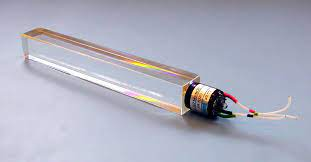
\includegraphics[width=0.8\textwidth]{figure/cms_crystal.jpeg}
    \caption[Photogram of a homogeneous lead tungstate crystal in the EE.]
    {Photogram of a homogeneous lead tungstate crystal in the EE, where the end of the crystal is a vacuum phototriode (VPT) photodetector.}
    \label{fig:cms_crystal}
\end{figure}

The ECAL consists of barrel section and two endcap sections assembled pointing towards the interaction point, shown in Fig.~\ref{fig:cms_ecal}.
The barrel section (EB) is composed of 61 200 individual crystals made in long geometries, $2.2\times 2.2\times 23 \mathrm{cm}^3$ covering $|eta|<1.479$.
The crystals allow total internal reflections to guide the scintillation light naturally to the photodetectors with the high refractive index ($n=2.29)$.
Modules are situated with an inner radius of 1.29 m and angular coverage up to $|\eta|=1.479$ in the barrel region.
In the endcap section (EE), the 3662 crystals for each endcap are arranged in a rectangular $x-y$ grid and are made in $3\times 3\times 22\mathrm{cm}^3$ extending the angular coverage up to $|\eta|<3$.
Endcap modules are positioned with the angular coverage of $1.479 < |\eta| < 3.0$. 
These crystals point at a focus 1300 mm beyond the center of the CMS detector, giving off-point angle ranging from 2 to 8 degrees.
The preshower detector (ES) is seated, just before the endcap, at $1.653 < |\eta| < 2.6$.
It is a silicon detector with a lead absorber aimed to enhance the spacial resolution to the endcap ECAL detectors, especially for distinguishing photons from boosted $\pi_0$ whose diphoton decay can be mis-identified with a single photon.
It is worthwhile mentioning that there is a small gap in the barrel-endcap region $|\eta| \in [1.4476, 1.5564]$, where is lack of crystals.
These regions are known to have poor resolution in particle reconstruction, and this region of the detector will not be used for precision measurements.
\begin{figure}[H]\centering
    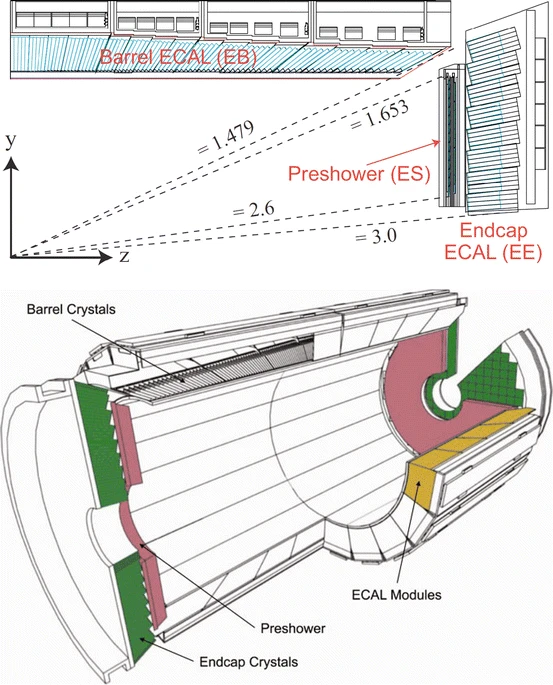
\includegraphics[width=0.7\textwidth]{figure/cms_ecal.png}
    \caption[Schematic view of the ECAL subsystem.]
    {Schematic view of the ECAL subsystem, including the barrel ECAL (EB), endcap ECAL (EE), and preshower (ES) subsystem.}
    \label{fig:cms_ecal}
\end{figure}

During the data collection, the photodetectors, the avalanche photodiodes (APDs) in the EB and vacuum phototriodes (VPTs) in the EE, collect the scintillation light produced from crystals with energy deposited. 
Next, the electronic signals from the photodetectors are amplified by the multi-gain pre-amplifier, which provides three simultaneous analogue outputs digitized at 40 MHz by a 12-bit analog-to-digital converter (ADC).
These digitized and filtered signals are then transmitted to off-detector with Level-1 trigger for further management.
The ECAL performance, the barrel energy resolution~\cite{Adzic:2007mi}, can be measured from an electron test beam experiment and decoupled into three terms as
\begin{linenomath}\begin{equation}\label{eq:cms_ecal}
    \frac{\sigma_E}{E} = \frac{2.8\%}{\sqrt{E(\GeV)}} \bigoplus \frac{12\%}{E(\GeV)} \bigoplus 0.3\%
\end{equation}\end{linenomath}
where the electron energy is reconstructed by the shower in $3\times 3$ crystals.
The first term of the equation is the stochastic term coming from shower containment, number of photoelectrons and fluctuations in the gain process.
The middle term is the noise term contributed by the photodetector electronics.
The last one, the constant term, dominating in high energy photon and electron showers, depends on non-uniformity of the longitudinal light collection, energy leakage from the back of the calorimeter, single-channel response uniformity and stability.

\subsection{Hadronic calorimeter (HCAL)}
The HCAL detector situated outside the ECAL aims to measure the energy of the hadrons and indirectly estimation of the presence of neutrinos.
It is in charge of the reconstruction of the jets originating from quark and gluon fragmentation and hadronization, and is designed as an array of sampling detectors, which strips the energy of the incoming particles with an absorber producing a shower of lower-energy secondary particles.
The scintillating materials then absorb those secondary particles for energy measurements.
The absorber materials used in the CMS detector consists of steel at the very front and back of each tower, and 14 layers of brass in between.
The thickness of the steel layer is 40 mm and 75 mm for the front and back plates, respectively.
The brass layers have a thickness varying from 50.5 mm to 56.5 mm with $70\%$ Cu and $30\%$ Zn, with a radiation length of 1.49 cm and a interaction length of 16.42 cm.

The HCAL detector is separated into the barrel part and the endcap part as with previous subdetector configurations shown in Fig.~\ref{fig:cms_hcal}.
The barrel part (HB) covers $|\eta|<1.4$ composed of 17 layers of active plastic scintillator tiles, giving a granularity of $0.087 \times 0.087$.
The innermost and outermost absorber layers are mode of stainless steel for structural strength.
The effective thickness absorber of the HB are increased with the polar angle from $5.82 \lambda_I$ to $10.6 \lambda_I$.
Since the hadronically interacting particles are not expected to be fully captured by the 17 layers of absorption material, an outer system (HO) placed just outside the solenoid is designed to use the solenoid and magnet iron yokes as an absorption material.
The total effective length can be further extended to a maximum of $11.8 \lambda_I$ in the central region.
The endcap part (HE) with the angular coverage of $1.3 < |\eta| < 3.0$ is with 19 layers of active plastic scintillator, giving granularity of $0.087 \times 0.087$ in $1.3 < |\eta| < 1.74$ and $(0.09 - 0.35) \times 0.087$ in $1.74 < |\eta| < 3.0$.
The average granularity is higher than HB, with a total effective length approximate to $10 \lambda_I$.
The forwards system (HF) is situated further along the beam line at 11.2 m from the center of the CMS detector and covers $3.0 < |\eta| < 5.2$ region.
The HF composed of steel absorbers in a cylindrical structure with radiation hard quartz fibers inserted is designed to measure the particles in the extreme $\eta$ regions.

The HCAL operates when a hadron particle passes through successive layers of absorber producing an amount of secondary particles.
The blue-violet light emitted by these secondary particles passing through the alternating layers of active scintillation is collected by optical wavelength-shifting fibers and shifted into green light.
A green optic signal is then sent by the normal optic cables to the front-end electronics where the optical signal is transformed into fast electronic signals by hybrid photodiodes (HPDs).
The signals are finally sent to data acquisition system for event triggering.
The energy resolution of the combined calorimeter (ECAL and HCAL) can be measured from a test beam experiment~\cite{USCMS:2009fxn} as
\begin{linenomath}\begin{equation}\label{eq:cms_resol}
    \frac{\sigma_E}{E} = \frac{84.7\%}{\sqrt{E(\GeV)}} \bigoplus \bigoplus 7.4\%
\end{equation}\end{linenomath}
where the first term is a stochastic term and the last term is a constant term.

\begin{figure}\centering
    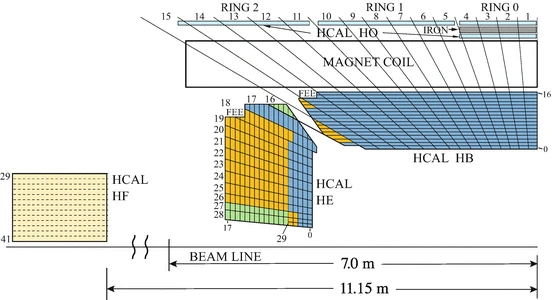
\includegraphics[width=0.9\textwidth]{figure/cms_hcal.png}
    \caption[Schematic view of the HCAL subsystem.]
    {Schematic view of the HCAL subsystem, including the barrel HCAL (HB), endcap HCAL (HE), outer HCAL (HO), and forward HCAL (HF) subsystem.}
    \label{fig:cms_hcal}
\end{figure}

\subsection{Magnet configuration}
The solenoid magnet, which give CMS its last name, is formed by a cylindrical superconducting coils with 6.4 m in diameter and 12.5 m in length making it the largest magnet of its type ever constructed.
It contains four layers of the coils made by Niobium-titanium for its high critical magnetic field and high critical current density.
The coils allows the current of 19.14 kA to flow without resistance while surrounded by 220 tonnes cold mass and cooled down to 4.7k to have no resistance.
The superconducting coils generate 3.8 T magnetic fields inside the detector, including the tracking system and calorimeters.
The job is to bend the paths of charged particle emerging from high-energy collisions for measuring their charges and momenta.

The tracker and calorimeter detectors fit snugly inside the magnet coil whilst the muon detectors are outside the solenoid.
A non-uniform and sparse flux caused by the return magnetic field outside the solenoid could lead ambiguous bending of muons, especially high-energy muons, and worsen the momentum resolution of the muon detectors.
A 12-sided steel flux-return yoke structure with a weight of 12 500 tonne is interleaved between the muon chambers to guide the magnetic and also acts as a filter, allowing through only muons and neutrinos. 
A complete distribution of the magnetic field strength for the magnet is shown in Fig.~\ref{fig:cms_magnet}
\begin{figure}\centering
    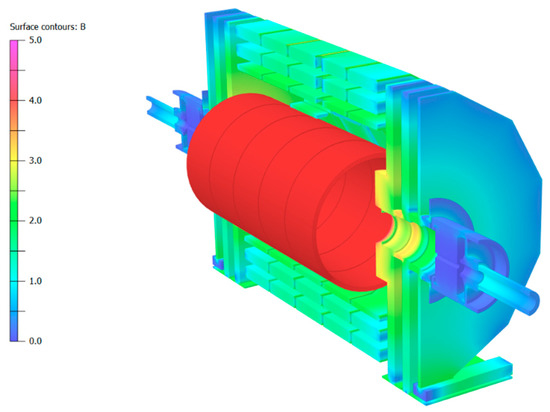
\includegraphics[width=0.8\textwidth]{figure/cms_magnet.jpg}
    \caption[Diagram of the solenoid magnet system in the CMS detector.]
    {Diagram of the solenoid magnet system in the CMS detector with the color scale corresponding to the interval of the magnetic flux density.}
    \label{fig:cms_magnet}
\end{figure}

\subsection{Muon detectors}
Due to the high mass of muons compared with the electrons, the bremsstrahlung radiation is relatively small, and thus muons are expected to penetrate all detector material in the calorimeter system.
Given this unique property, muons are expected to be one of the clearest signature for high energy events.
Precision measurements of muons outside the existing detectors is performed by muon detectors situated outside the outer HCAL system and the solenoid magnet.
A gas-chamber type of detector~\cite{CMS:mu_PF} is designed to reconstruct the muon information with the angular coverage of $|\eta| < 2.4$.
The muon detectors are composed of three different gas ionization chambers, the drift tube chambers (DT), cathode strip chambers (CSC), and the resistive plate chambers (RPC), as shown in Fig.~\ref{fig:cms_muon}.
All the different muon systems share the same sensor operating principle.
The anode and cathode maintained at high voltage differences are interleaved with an inert gas.
Muons passing through this sensor would ionise the gas, which then drift to the anode and cathodes, producing a measurable current at the anode and cathode.
\begin{figure}\centering
    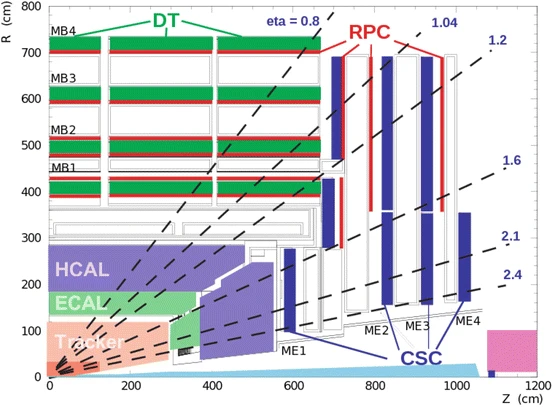
\includegraphics[width=0.7\textwidth]{figure/cms_muon.png}
    \caption[Schematic view of the muon subsystems in the $r-\eta$ plane.]
    {
        Schematic view of the muon subsystems in the $r-\eta$ plane. 
        Cathode strip chambers are in red.
    }
    \label{fig:cms_muon}
\end{figure}


The DTs are placed in the barrel region $|\eta| < 1.2$ where muon rates are expected to be lower, with the basic elements of standard rectangular cells containing four electrodes for shaping the effective drift filed(Fig~\ref{fig:cms_cell}.
The DT cells with a size of 42 mm $\times$ 13 mm $\times$ 2.4 m are layered with the cathode as aluminium tape, and a single gold-plated stainless-stell anode is centered inside each tube shaping the effective drift field with four electrodes.
The anode receives the induced electrons in the inert gas composed of $85\%$ Ar and $15\%$ $\mathrm{CO_2}$ at a drift velocity of about 55$\mu$m/ns when muons go through the cell and ionize the gas.
A DT chamber is made of three superlayers, and a superlayer is composed of three DTs, as in Fig.~\ref{fig:cms_DT}.
\begin{figure}\centering
    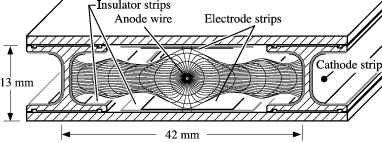
\includegraphics[width=0.8\textwidth]{figure/cms_cell.png}
    \caption[Layout of a DT cell.]
    {Layout of a DT cell, showing the electric field lines in the gas volume.}
    \label{fig:cms_cell}
\end{figure}

\begin{figure}\centering
    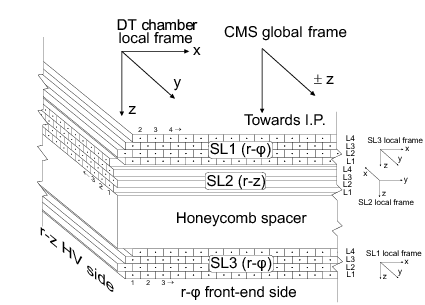
\includegraphics[width=0.7\textwidth]{figure/cms_DT.png}
    \caption[Schematic layout of a DT chamber.]
    {
        Schematic layout of a DT chamber. 
        The SL1 and SL3 superlayers measure the $r-\phi$ coordinate in the bending plane of CMS.
        The SL2 superlayer measures the $z$ coordinate, along the direction parallel to the beam.
    }
    \label{fig:cms_DT}
\end{figure}

Due to the high muon rate and non-uniform magnetic field, the CSC with fast response time is located in the endcaps of the CMS detector.
It covers a region of $0.9 < |\eta| < 2.4$ providing good timing and spacial resolution.
Each CSC consists of 6 anode wire plans interleaved with 7 cathode panels, as shown in Fig.~\ref{fig:cms_CSC}.
The cathode panel are configured as stripes along the radial direction contains 80 cathode strips.
In contrast, the anodes are configured as thin wires with a diameter of 50 $\mu$m on the anode planes along the azimuthal direction.
The anode wire plans are filled with 6 gas gaps in between, each of which is full of a mixture of $50\% \mathrm{CO_2}$, $40\%$ Ar and $10\% \mathrm{CF_4}$.
With the structure mentioned above, the CSCs provide 2 dimensional 2 dimensional information of the muon position within a single chamber module, when the currents of both cathode and anode are measured.
\begin{figure}\centering
    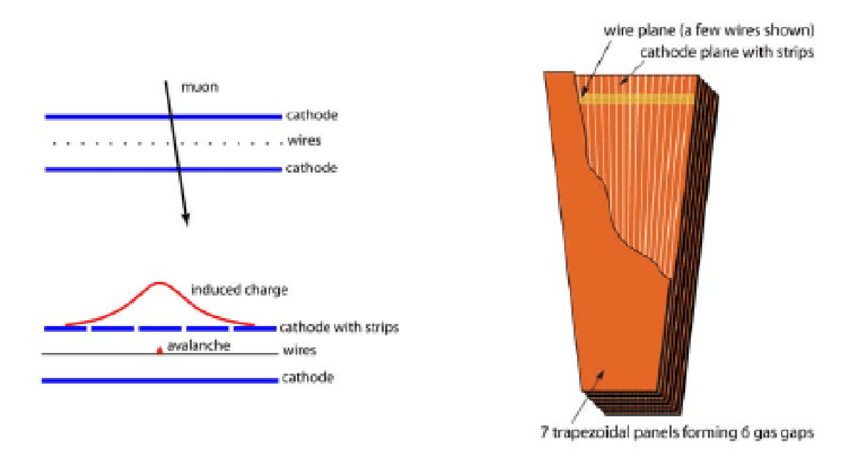
\includegraphics[width=0.85\textwidth]{figure/cms_CSC.png}
    \caption[The layout of CSC system in the CMS.]
    {The layout of a cathode strip chambers (right) and a cross-sectional views of the gas gap in a CSC gap with the anode wires and cathode planes  (left).}
    \label{fig:cms_CSC}
\end{figure}

Besides the DTs and CSCs, the RPC, a trigger-based detector system, is placed outside in both barrel and endcap regions providing adequate timing information for keeping the muon system in sync with the other subdetectors.
Each RPC is made of two gaps composed of highly resistive Bakelite plastic filled with a mixture of $95.2\% \mathrm{C_2H_2F_4}$, $4.5\% \mathrm{i-C_4H_{10}}$ and $0.3\% \mathrm{SF_6}$ in between (Fig.~\ref{fig:cms_RPC}, to keep the drifting electrons and ions from the ionised gases away from the anode and cathode.
The conductive graphite layer on the outer surface of the resistive plates provides avalanches which is sent to the readout strips to form a signal, when charged particles pass through a RPC and ionize the gas.

\begin{figure}\centering
    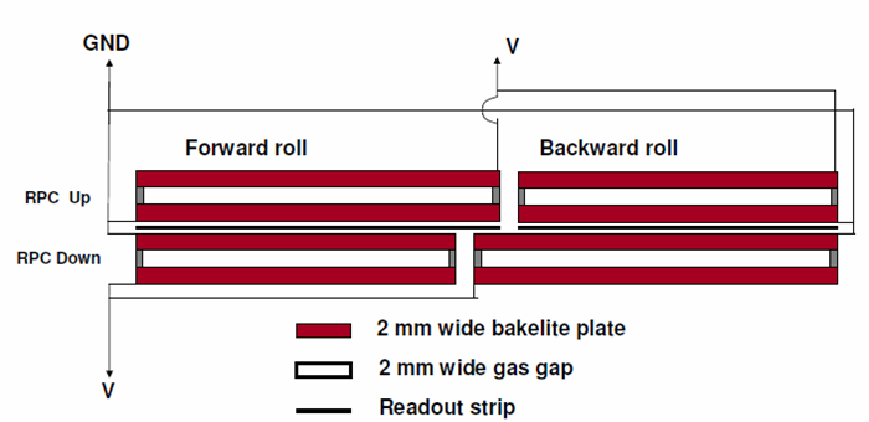
\includegraphics[width=0.85\textwidth]{figure/cms_RPC.png}
    \caption{Schematic view of a generic barrel RPC with 2 roll partitions.}
    \label{fig:cms_RPC}
\end{figure}

